\documentclass[a4paper, 11pt]{article}
    \usepackage[left=2cm, top=3cm, text={17cm,24cm}]{geometry}
    \usepackage[utf8]{inputenc}
    \usepackage[T1]{fontenc}
    \usepackage{times}
    \usepackage{graphics}
    \usepackage{subcaption}
    \usepackage{hyperref}
    \pdfminorversion=7


\begin{document}

\begin{titlepage}
    \begin{center}
        \textsc{\Huge{Brno University of Technology\\[0.4em]}
        \huge{Faculty of Information Technology}}\\        
        \vspace{\stretch{0.382}}
        \huge{\textbf{Documentation of compiler for language \textsc{IFJ24}}}\\
        \LARGE{Team xnovakf00\,--\,variant vv-BVS}\\
        \Large{extensions: \textsc{funexp}}\\
        \vspace{\stretch{0.618}}
    \end{center}
    \Large{Matúš Fignár xfignam00\,--\,25\%\\
            Tibor Malega xmalegt00\,--\,25\%\\
            Filip Novák xnovakf00\,--\,team leader\,--\,25\%\\
            Ján Skovajsa xskovaj00\,--\,25\%\hfill \today}
\end{titlepage}

\tableofcontents
\newpage
\listoffigures
\newpage

% ODTADE PISTE CO CHCETE, KED CHCETE ODSEK POUZITE \section{NAZOV}, KED PODODSEK \subsection{NAZOV},
% ESTE MENSI TA \subsubsection....
% KOMENTARE CEZ %

% KED KOD/NIECO TECHNICKE tak \verb | TEXT |
% KED VSETKO VELKYM (AKO NAPR FUNEXP NA TITULKE) TAK \textsc{TEXT}
% HRUBE \textbf{TEXT}
% ITALICS \textit{TEXT}
% KEBY HOCICO INE POTREBUJETE TAK TAG ME

\section{Design and implementation of the compiler}
Compiler uses double-traversal method of the source code based on "top-down" recursive parsing specified by
LL(1) grammar\footnote{See figures \ref{ll1rules} and \ref{ll1table}.}. Expressions are processed using precedence syntactic
analysis. Lexical analyser (scanner) processes source code and tokenizes it based on deterministic finite automaton\footnote{See figure \ref{automaton}.}.
During parsing, semantic analysis is performed and abstract syntax tree (AST) is constructed for internal representation.
Compiler uses table of symbols, implemented as height-balanced binary search tree for keeping information about defined functions and variables.
Code is generated through recursive traversal of constructed AST.

\section{Lexical analysis}\label{sec:LEX}

\section{Syntactic analysis}\label{sec:SYNTACTIC}
Syntactic analysis is divided into two parts\,--\,expression parser and
recursive parser processing the rest of the source code. These two are closely intertwined.
Both call scanner to receive tokens to evaluate.\par
When recursive parser expects an expression in source code (denoted as \verb|expression| in LL(1) grammar~(\ref{ll1rules})), 
expression parser is called for processing.
\subsection{"Top-down" syntactic analysis}\label{sec:PARSER}
Recursive parser is implemented as a set of functions, each representing certain non-terminal of LL(1) grammar, found in
\verb|parser.c, parser.h|.
Functions validate sequence of tokens received by invoking scanner with function \verb|getToken()| (or macro \verb|GT| for 
compactness). When another non-terminal is expected, function representing it is called.
Each function returns \verb|0| when processing of the non-terminal was successful. If an error occurs, \verb|ERROR| is called\footnote{See section
about errors \ref{sec:ERR}.}.
\par
In the first traversal, information about user-defined functions are collected. This includes:
\begin{itemize}
\item function IDs
\item return data types
\item number of parameters
\item parameter names 
\item parameter data types
\end{itemize}
Other tokens, not representing function headers are skipped 
.This is implemented as loop with break condition being encountering token \verb|pub|, signaling start of the next function definition.
\par
Second traversal performs regular parsing of the source code with validation of token sequence, performing semantic analysis and constructing
AST.
\par
To support double traversal, function processing user-defined functions was split into two separate with 
adjusted logic: \verb|def_func_first()| and \verb|def_func_sec()|. For readability and reusability, \verb|after_id|~
function was split into two parts: \verb|funCallHandle()|, processing standalone function calls in source code (or function calls 
in expressions) and \verb|assignmentHandle()|, processing assignment to variables.
\par
Validating compulsory prologue in source code is handled in LL(1) grammar as rule 2. For simplicity, 
\verb|ifj| namespace and string literal \verb|"ifj24.zig"| are represented as id terminal and expression.
Further validation of their correctness is done in \verb|prog()|. If either of them is incorrect, syntax error
is raised and program exits with error code \verb|2|.

\subsection{"Bottom-up" syntactic analysis of expressions}\label{sec:EXPRPARSER}

\section{Semantic analysis}\label{sec:SEMANTIC}
ADD TEXT
\subsection{Semantic analysis in "top-down" parser}
\subsubsection{Variables}
When defining a variable, parser ensures no \textbf{redefinition} of already
existing variable occurs within the same nested blocks. This is achieved by searching stack using
\verb|findInStack()|. If \verb|NULL| is returned, redefinition is not detected. Similarly,
\verb|funSymtable| is also searched for an entry with matching ID.
\par Assignment to \textbf{undefined variables} are not allowed. Verification is similar to redefinition check,
however non-\verb|NULL| value is expected.
\par \textbf{Matching data types} of the variable and the assigned expression in assigning and defining must be confirmed.
This is done by examining data type of the \verb|astNode| representing expression. Expression cannot be logical.
\par As explicit data type of a variable during definition can be omitted, it is necessary to \textbf{inherit data type
from expression}. If it is not possible (e.g. expression is \verb|null| or \verb|string| literal), an error is raised.
If the data type can be deduced, it is set to symbol table entry of a variable along with nullability of the variable.
\par When parser is finished with processing block of code bounded with curly brackets, symbol table on the top of the stack
is recursively traversed (preorder traversal, function \verb|allUsed()|) and flags \verb|changed| and \verb|used| are observed,
ensuring that \textbf{all modifiable variables were modified} and \textbf{all defined variables within block were used}. This includes
\verb|id_without_null| in \textit{if-else} and \textit{while} as well as function parameters.

\subsubsection{Functions}
\textbf{Redefinition of functions} is checked during the first traversal of the parser (same concept as variable redefinition check).
With separate symbol table for built-in functions, matching IDs are allowed (e.g. \verb|ifj.write()| and user-defined \verb|write()|).
\par
Validation that all user-defined functions are \textbf{used within program} is performed at the very end of second traversal of parser,
by examining \verb|used| flag in \verb|funSymtable| nodes. Function \verb|main()| has this flag set to \verb|true| implicitly. 
\par
\textbf{Non-void function not containing any return statements} in all possible execution paths is evaluated as semantic error.
This is analysed by \verb|allReturns()| function, using depth-first recursive traversal of AST of a function body.
Function returns \verb|true|, if:
\begin{itemize}
    \item \verb|return| AST node is encountered
    \item all paths in \verb|if| and \verb|else| blocks return true
    \item all paths in \verb|while| block return true
\end{itemize}
When a different AST node is encountered, \verb|allReturns()| is called on the \verb|next| of the AST node.
\par
\textbf{Type compatibility in returning expression} is checked with each \verb|return| statement. If it is not compatible with
expected return type (from function definition), error is raised. Similarly, when a \verb|void| function returns an expression,
error is raised.
\par
When a function is called outside of an expression, it must be \verb|void|. Return type of function is examined in 
symbol table entry.
\par
\textbf{Presence of main function} in source code is validated by \verb|mainDefined()| at the end of first traversal.
At the same time, \textbf{parameters and return type of main} are checked, ensuring they match the expected specification.

\subsubsection{Other semantic checks}
When \verb|while| or \verb|if-else| statements are being processed by parser, condition expression is checked.
In statements without the nullable variable part, logical expression is expected. In statements with \verb|id_without_null|,
condition has to be nullable.

\section{Table of symbols}\label{sec:SYMTABLE}
Data structure representing symbol tables in implementation is \textit{height-balanced binary search tree}.
Functions for working with symbol tables, structs representing nodes or node data and functions for printing
.dot visualisation of symbol table can be found in \verb|symtable.c| and \verb|symtable.h|. Recursive approach was adopted because the binary tree itself is recursive in nature.
\par
Compiler utilizes three distinct types of symbol tables: 
\begin{itemize}
    \item symbol table for user-defined functions
    \item symbol table for built-in functions
    \item symbol table for defined variables
\end{itemize}
 For all types, ID of an element, represented as
an array of characters, is used as key based on which the tree is arranged. Node representation (\verb|struct symNode|) is the same for all, one thing that varies
is data representation in union \verb|data| (\verb|struct funData| for functions and \verb|struct varData| for variables).
\subsection{User-defined functions}
Symbol table for \textbf{user-defined functions} is a global variable \verb|symtable funSymtable| declared in \newline\verb|symtable.h|. Parser calls
\verb|createSymtable()| to initialise it. Nodes include information collected during first traversal of parser and pointer 
to a symbol table for variables defined within the function.
\subsection{Built-in functions}
Symbol table for \textbf{built-in functions} is also a global variable \verb|symtable builtinSymtable| declared in \verb|symtable.h| sharing
the same information as symbol table for user-defined functions. It is populated by parser using function \verb|prepareBuiltinSymtable()|.
All data are pre-initialised based on assignment. No new entry is added into this function after initialisation\,--\,it is only used
for semantic checks and AST construction. 
\par For built-in functions \verb|ifj.write(term)| and \verb|ifj.string(term)|, extra
data types (\verb|any, stringOru8|) in \verb|enum dataType| were introduced, as parameters in these functions can take multiple data types. 
\par Separation of symbol tables for built-in and user-defined functions was realised for support of user-defined functions with the same ID as an existing built-in one.
\subsection{Variables}
Symbol tables for \textbf{defined variables} are created during parsing of blocks of code bounded by curly brackets (functions, \textit{while} and \textit{if-else}).
Scopes, in which defined variable is accessible are implemented using stack of symbol tables (global variable \verb|stack symtableStack|).
Stack is implemented as singly linked list. Function \verb|findInStack()| is used to traverse symbol table stack and look for nodes with given key.
If no entry is found in the whole stack, \verb|NULL| is returned.


\section{Abstract syntax tree}\label{sec:AST}
Abstract syntax tree (found in \verb|ast.c, ast.h|) is implemented as acyclic graph with specialised node types to represent
different components of the source code.
The AST includes the following node types, each representing a specific syntactic construct: 
\newline
\noindent
\begin{minipage}[t]{0.3\textwidth}
\begin{itemize}
    \item \textbf{Control Flow}
    \begin{itemize}
        \itemsep-0.1em
        \item while
        \item if-else
        \item if
        \item else
    \end{itemize}
\end{itemize}
\end{minipage}%
\begin{minipage}[t]{0.3\textwidth}
\begin{itemize}
    \item \textbf{Statements}
    \begin{itemize}
        \itemsep-0.1em
        \item assign
        \item unused declaration
        \item variable definition
        \item function definition
        \item return
    \end{itemize}
\end{itemize}
\end{minipage}
\begin{minipage}[t]{0.3\textwidth}
\begin{itemize}
    \item \textbf{Expressions}
    \begin{itemize}
        \itemsep-0.1em
        \item expression
        \item binary operator
        \item function call
        \item literal
        \item variable
    \end{itemize}
\end{itemize}
\end{minipage}
\newline
\par
Each node has distinct set of information needed for semantic analysis or code generation, implemented with
\verb|struct|. Nodes may include pointer to a different nodes (e.g. condition in \textit{while} or \textit{if-else}, expression node in assign or return).
All nodes in constructed AST are \verb|struct astNode|, which serves a purpose of general representation.
Information included in \verb|astNode|:
\begin{itemize}
    \item type of node
    \item pointer to the next statement in block (in case node itself represent a statement)
    \item union of node representations (exact representation of a node, as mentioned before)
\end{itemize}

Each node type has a designated function for its creation (\verb|create*Node()|, where \verb|*| is the type of the node)
with all information needed to be stored as parameters.
\par Special node \verb|root| only includes a \verb|next| pointer, which serves as a connecting piece for
bodies of functions, \textit{if-else} or \textit{while}. Global variable \verb|AST ASTree|, declared in \verb|main.c| is an
encapsulation of the \verb|root| of the AST of the whole source code. It is the product of syntactic analysis.
\par  Functions for printing .dot representation for visualisaton of AST are also implemented.

\section{Code generation}\label{sec:CODEGEN}

Code generation was performed by traversing the \textsc{Abstract Syntax Tree} (AST). This traversal involved an iterative approach for the overall structure and recursive processing for function bodies.

\subsection{Code Buffer}

For code generation, an additional data structure, \verb|Buffer_ll|, was developed and implemented in the modules \verb|code_buffer.h| and \verb|code_buffer.c|. The \verb|Buffer_ll| structure is designed as a linked list where each node contains a pointer to a string, typically representing one line of code. Exceptions include cases like generating headers or built-in functions.

The \verb|Buffer_ll| also incorporates:
\begin{itemize}
    \item A pointer to an \textbf{accumulator string} for temporarily storing a string before adding it to a node.
    \item A special pointer, \verb|flag|, that marks a specific node. This allows inserting a new node after the flagged node instead of appending it to the end of the list. This feature was primarily used for managing variable declarations.
\end{itemize}


\subsection{Header and Built-In Functions}

At the start of code generation, a header is generated. This includes:
\begin{itemize}
    \item The declaration of the intermediate code header: \verb|.IFJcode24|.
    \item Global variable declarations for storing function return values.
    \item Proper initialization for code execution.
\end{itemize}

Next, built-in functions without a direct representation in \verb|IFJcode24| are implemented as standalone functions. These built-in functions are prefixed with \verb|$$| to differentiate them from user-defined functions and keywords in \verb |IFJcode24|. Other built-in functions, which correspond directly to \verb|IFJcode24| instructions, are generated when called, primarily for optimization purposes.

\subsection{User-Defined Functions}

User-defined functions are prefixed with \verb|$| to distinguish them from built-in functions and keywords in \verb|IFJcode24|. After generating the corresponding label for a function, the code generator flags a node in \verb|Buffer_ll|. This enables the declaration of all variables that are used in function at the beginning of the function, ensuring that in generated code will be no reinitialization. Note that reinitialization is not supported in \verb|IFJcode24|. 

For every user-defined variable, compiler adds the prefix \verb|_| to differentiate it from other variables used by the compiler for various purposes.

Function bodies are generated recursively by traversing the \textsc{AST} and producing the corresponding code for each node.

\subsection{Generating \textit{if} and \textit{while} Statements}

For generating \textit{if} and \textit{while} statements, unique labels are required throughout the generated code. To achieve this:
\begin{itemize}
    \item A static variable, \verb|count|, is used to store the number of generated labels.
    \item Before generating a new statement, \verb|count| is incremented.
    \item A special function is called to generate a unique and relevant label for the statement.
\end{itemize}

\subsection{Expressions}

Expressions are generated using a stack, which supports \verb|IFJcode24| instructions. This approach simplifies the processing of expressions derived from a binary tree. Expression generation involves:
\begin{itemize}
    \item Traversing the top-level binary tree for expression recursively using \textit{post-order} traversal.
    \item For binary operators, invoking the corresponding \verb|IFJcode24| instruction ensures the correct order of values is maintained in the stack.
\end{itemize}

This design ensures efficient and reliable processing of expressions during code generation.


\section{Error handling and memory management}\label{sec:ERR}

\section{Teamwork}\label{sec:TEAM}
Implementing a compiler is not an easy task, that is why the work has begun as soon as 
the assignment was published. Firstly, tasks were distributed among all members based on 
preferences.\par 
Test submission was set as deadline for implementation. This deadline
was successfully met with time left for fixing errors and further testing. Pair programming as well as 
code reviews were practised. 

\subsection{Communication}\label{sec:COMM}
Discord was chosen as primary mean of communication. In specialised voice and text channels meetings were
held at least once a week. Git was used as versioning system with remote repository hosted by team leader at
GitHub. Using webhook, Discord bot for notifications about changes on remote repository was added.\par
Email addresses and telephone numbers were shared among all members in case of an unexpected situation.
Luckily, no problems were encountered and communication ran smoothly for the whole duration of the project.

\subsection{Task distribution}\label{sec:TASKS}
\begin{itemize}

    \item \textbf{Matúš Fignár xfignam00}\,--\,precedence table, "bottom-up" expression parsing
    \item \textbf{Tibor Malega xmalegt00}\,--\,finite automaton design, lexical analysis
    \item \textbf{Filip Novák xnovakf00}\,--\,"top-down" recursive parsing, table of symbols, testing, AST
    \item \textbf{Ján Skovajsa xskovaj00}\,--\,code generation, testing

\end{itemize}
The remaining parts of the project were developed by all members of the team simultaneously.














\newpage
\section{Attachments}
\begin{figure}[ht]
    \begin{center}
        \scalebox{0.25}{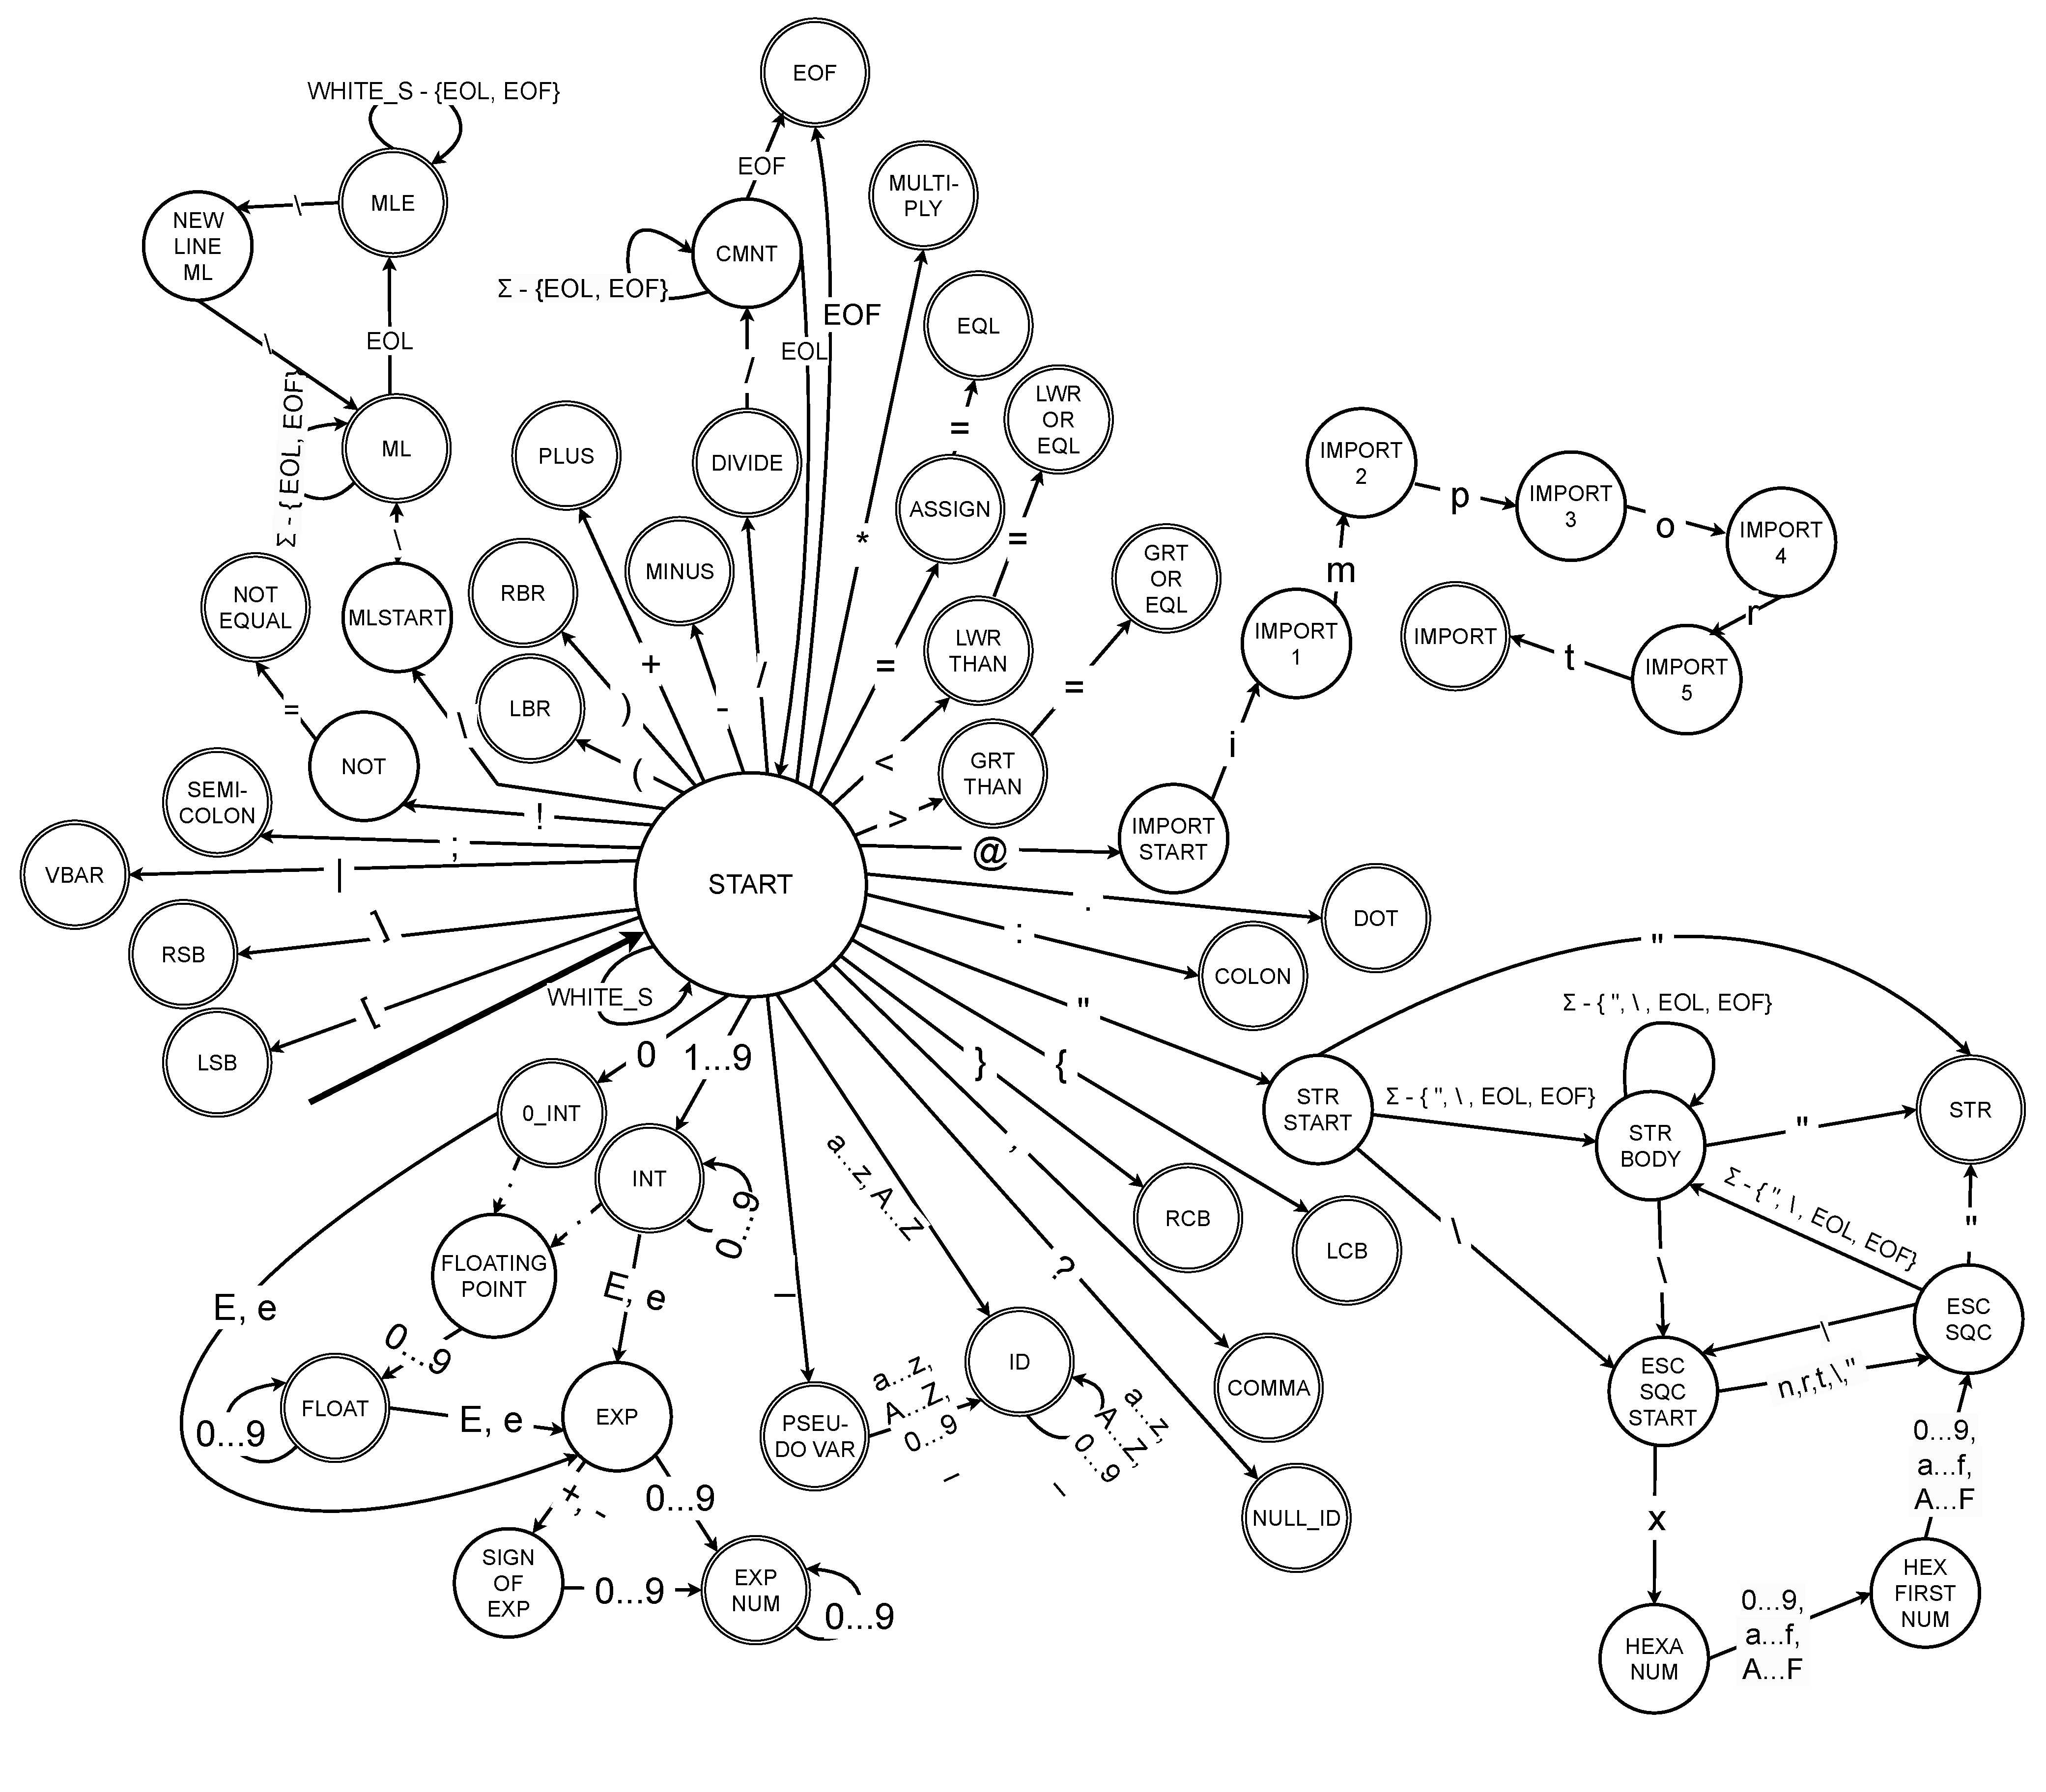
\includegraphics{doc/automaton.pdf}}
        \caption{Deterministic finite automaton for lexical analysis}
        \label{automaton}
    \end{center}
\end{figure}

\begin{figure}[ht]
    \begin{center}
    \begin{enumerate}
        \itemsep-0.5em
        \item \textless prog\textgreater\  $\to$ \textless prolog\textgreater\ \textless code\textgreater
        \item \textless prolog\textgreater\ $\to$ const id = @import ( expression ) ;
        \item \textless code\textgreater\ $\to$ \textless def\_func\textgreater\ \textless code\textgreater
        \item \textless code\textgreater\ $\to$ $\varepsilon$
        \item \textless def\_func\textgreater\ $\to$ pub fn id ( \textless params\textgreater ) \textless type\_func\_ret\textgreater\ \{ \textless body\textgreater \}
        \item \textless params\textgreater\ $\to$ id : \textless type\textgreater\ \textless params\_n\textgreater
        \item \textless params\textgreater\ $\to$ $\varepsilon$
        \item \textless params\_n\textgreater\ $\to$ , \textless params\textgreater
        \item \textless params\_n\textgreater\ $\to$ $\varepsilon$
        \item \textless def\_variable\textgreater\ $\to$ \textless varorconst\textgreater\ id \textless type\_var\_def\textgreater\ = expression ;
        \item \textless varorconst\textgreater\ $\to$ const
        \item \textless varorconst\textgreater\ $\to$ var
        \item \textless unused\_decl\textgreater\ $\to$ \_ = expression ;
        \item \textless type\_normal\textgreater\ $\to$ i32
        \item \textless type\_normal\textgreater\ $\to$ f64
        \item \textless type\_normal\textgreater\ $\to$ [ ] u8
        \item \textless type\_null\textgreater\ $\to$ ? \textless type\_normal\textgreater
        \item \textless type\textgreater\ $\to$ \textless type\_normal\textgreater
        \item \textless type\textgreater\ $\to$ \textless type\_null\textgreater
        \item \textless type\_func\_ret\textgreater\ $\to$ \textless type\textgreater
        \item \textless type\_func\_ret\textgreater\ $\to$ void
        \item \textless type\_var\_def\textgreater\ $\to$ : \textless type\textgreater
        \item \textless type\_var\_def\textgreater\ $\to$ $\varepsilon$
        \item \textless expr\_params\textgreater\ $\to$ expression \textless expr\_params\_n\textgreater
        \item \textless expr\_params\textgreater\ $\to$ $\varepsilon$
        \item \textless expr\_params\_n\textgreater\ $\to$ , \textless expr\_params\textgreater
        \item \textless expr\_params\_n\textgreater\ $\to$ $\varepsilon$
        \item \textless after\_id\textgreater\ $\to$ = expression ;
        \item \textless after\_id\textgreater\ $\to$ \textless builtin\textgreater\ ( \textless expr\_params\textgreater ) ;
        \item \textless assign\_or\_f\_call\textgreater\ $\to$ id \textless after\_id\textgreater
        \item \textless builtin\textgreater\ $\to$ . id
        \item \textless builtin\textgreater\ $\to$ $\varepsilon$
        \item \textless st\textgreater\ $\to$ \textless def\_variable\textgreater
        \item \textless st\textgreater\ $\to$ \textless assign\_or\_f\_call\textgreater
        \item \textless st\textgreater\ $\to$ \textless unused\_decl\textgreater
        \item \textless st\textgreater\ $\to$ \textless while\_statement\textgreater
        \item \textless st\textgreater\ $\to$ \textless if\_statement\textgreater
        \item \textless st\textgreater\ $\to$ \textless return\textgreater
        \item \textless body\textgreater\ $\to$ $\varepsilon$
        \item \textless body\textgreater\ $\to$ \textless st\textgreater\ \textless body\textgreater
        \item \textless return\textgreater\ $\to$ return \textless exp\_func\_ret\textgreater  ;
        \item \textless exp\_func\_ret\textgreater\ $\to$ $\varepsilon$
        \item \textless exp\_func\_ret\textgreater\ $\to$ expression
        \item \textless id\_without\_null\textgreater\ $\to$ | id |
        \item \textless id\_without\_null\textgreater\ $\to$ $\varepsilon$
        \item \textless while\_statement\textgreater\ $\to$ while ( expression ) \textless id\_without\_null\textgreater\ \{ \textless body\textgreater \}
        \item \textless if\_statement\textgreater\ $\to$ if ( expression ) \textless id\_without\_null\textgreater\ \{ \textless body\textgreater \} else \{ \textless body\textgreater \}
    \end{enumerate}
    \caption{LL(1) rules}
    \label{ll1rules}
\end{center}
\end{figure}

\begin{figure}[ht]
    \begin{center}
        \scalebox{0.6}{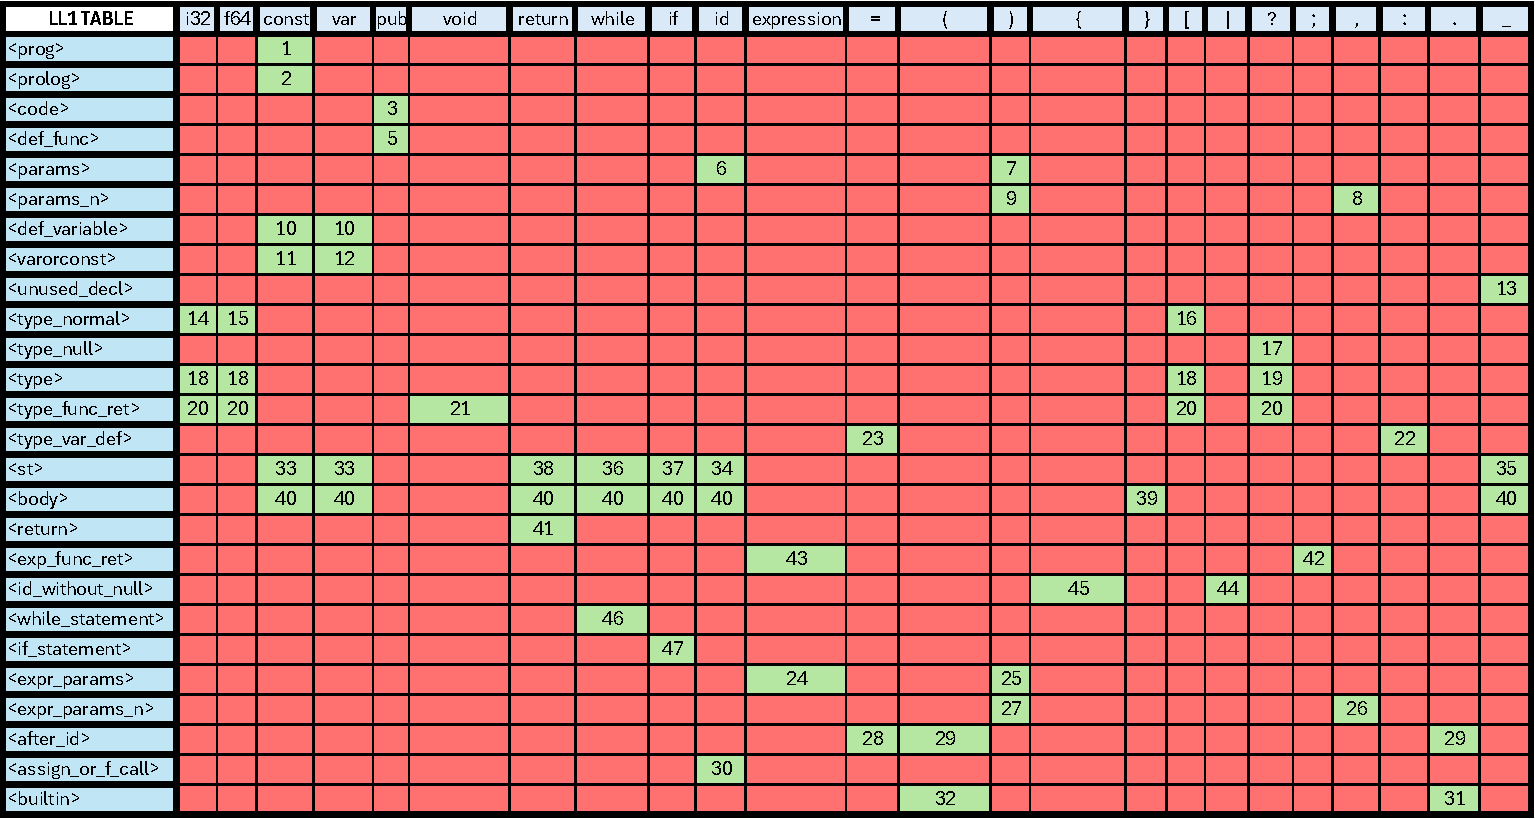
\includegraphics{doc/LL1_table.pdf}}
        \caption{LL(1) table for parsing}
        \label{ll1table}
    \end{center}
\end{figure}

\end{document}